%!TEX root = ../../main.tex
%----------------------------------------------------------------------------
\chapter{System Test}\label{chap:system_test_chapter}
%----------------------------------------------------------------------------

% Please keep sections separated in their designated folders and only reference them here using the input tag

In order to prove the capabilities of our design and to bring all the so far undetected bugs and errors to light, a $24$ hour integration test was required. During these $24$ hours, all components of the system had to be used throughout multiple iterations of the brick selection and delivery procedure. 

Since the timespan of the test was such that it encapsulated a whole day, the systems had to cope with changing light conditions, continuous interference by human operators and spectators moving around, degradation of navigation markers and the mobile platforms of the other groups. In the following sections a detailed description of the performed tests are present alongside the results and evaluation.

\section{Test description}
In the beginning of the test, all mobile platforms were situated at the charging stations, fully charged. One iteration consisted of the following milestones:

\begin{enumerate}
	\item Leaving the charging station in a fully charged state and taking up position under the LEGO dispenser machine
	\item Waiting for the bricks to be loaded on the tipper (since the dispenser was not operational, we just simulated the process)
	\item Delivering the LEGO to the robot cell
	\item Unloading the bricks to the conveyor belt
	\item Moving the bricks into position for selection through robotic vision
	\item Picking the LEGO bricks specified by the order (this is equivalent to loading them on the mobile platform)
	\item Transporting the LEGO back to the box, and docking at the charger
\end{enumerate}

All components of the system were continuously broadcasting location and status information, which was displayed on the HMI, while the map used for SLAM navigation and the console-printed ROS information were also monitored. We compared all these with the actual position and behaviour of the system components, logged their performance, and intervened when errors occurred. 

\section{Log}
The date and time was logged alongside the person responsible for creating the entry, the type of the entry and a short note describing the reason for making it.

The following types are distinguished between:

\begin{itemize}
	\item Order Start
	\item Order Finish
	\item Error
	\item Manual Shutdown
	\item System Event
	\item Other
\end{itemize}

\section{Test results}
Even though in the initial phase camera connection issues caused delays in the testing process, all in all $49$ iterations were performed, out of which $36$ were finished successfully resulting in a success ratio of $73.47\%$ (details see Figure \ref{fig:order_statistics}). The full log can be seen in Appendix \ref{"apx:log"}

\begin{figure}[H]
	\centering
	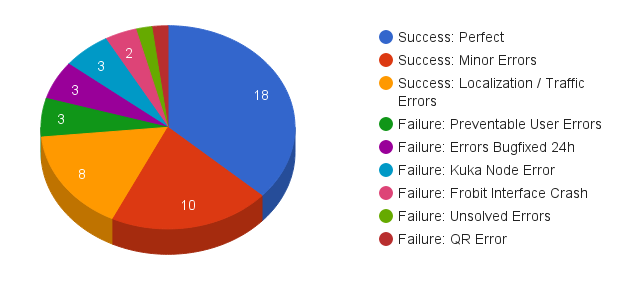
\includegraphics[width=0.9\textwidth]{stress_test_pie}
	\caption{Stress Test Results}
	\label{fig:order_statistics}
\end{figure}

The speed of the system was improved throughout the test and on average an execution time of $9.28$ minutes was achieved with a standard deviation of $3.35$. The highest factor in deviation in time as well as the highest error rate was due to localization errors and traffic jams inside and around the box. A combined MES-Server, that ensures only one robot moving around in the box would solve this issue completely. 
\newpage
\textbf{Major Lessons learned during $24$-hour stress test:}
\begin{itemize}
\item Protocol for recovery after breaking safety
\item Reboot procedure
\item Protocol for hot-swapping Battery
\item Maintain good QR-Quality
\end{itemize}

\textbf{Bugs fixed or improved during $24$-hour stress test:}
\begin{itemize}
\item Inverse Kinematics error detection and handling
\item Increased Kuka Speed
\item Adjusted required battery level to make one run
\item QR Codes replaced
\end{itemize}

\textbf{Open To-Do's before shipping:}
\begin{itemize}
\item Improve vision for better \textit{monster} recognition
\item Fix loose connections
\item Solve unloading issue
\item Solve Kuka Node crashing
\item Fix Frobit Interface Crashes
\item MR GO node crashed once, no reason / solution found
\end{itemize}

%%% Local Variables:
%%% mode: latex
%%% TeX-master: "main"
%%% End: